\chapter{MULTI-MODAL REASONING-BASED ROSL ALGORITHM}\label{chap:LLM}

% Multimodal models
    % Biology inspiration self-supervised learning models: MIT papers
    % Brief of which brain part does what, which one processes sensory inputs, comparable DL systems
    % How LLM is a brain-inspired candidate for navigation decision by reasoning over sensory inputs.
% proposed solution: generalized reasoning over detected objects with multimodal LLM
% how multimodal model works - not just object name, but with object context.
% the model is generalized, and has the ability to solve a specific problem

% LLM as the new paradigm in robotics
    % Brief of LLM
    % why is llm good for robotics
        % from literature
        % Biology inspiration: MIT papers
            % Brief of how brain makes sensory input based navigation
                % Which  brain part does what, comparing DL systems with them
                % How LLM is a brain-inspired candidate for navigation decision by reasoning over sensory inputs.

\section{Introduction}
\subsection{Background}\label{Subsec:LLMBackground}
% background (limitation of supervised vision model) and problem statement
The Fusion navigation algorithm discussed in chapter~\ref{chap:fusion} has shown to be effective at localizing the odor source in real-world environments with turbulent airflow and a few obstacles. But the vision sensing can only extract odor source location information if the odor source emits visible plume. The vision model doesn't extract any odor source location information if visible plume is absent, or the vision is blocked. However, there is latent information in the vision data that can help narrow search boundaries. For example, we may narrow our odor source search area to a restaurant without directly seeing the odor-emitting food. However, this requires the ability to reason over the search objective and the environment. It is difficult to train a supervised vision model to gain generalized reasoning capability.

Reinforcement Learning (RL) can be used to teach an agent the relationship between the given objective and the surrounding environment \cite{sutton2018reinforcement}. However, RL requires extensive training that may be unfeasible in the real-world environments. If the agent is trained in a simulated environment, the simulation needs to closely match the complexities of the real world to ensure effective transfer of learning to the real environment \cite{zhao2020sim}. Even after sufficient training for a given objective, the learnings may not be transferable to a new objective.

In contrast to supervised and reinforcement learning, Large Language Models (LLM) have reasoning capabilities. This allows them to extract information from previously unseen data for diverse objectives. This problem of environment understanding is a central theme of embodied AI research.

% related research (embodied AI and LLM based navigation)
\subsection{Related Research}\label{Subsec:LLMRelatedResearch}

Embodied Intelligence is a growing research area focused on intelligent agents that closely interact with their environment. The field hypothesizes that intelligence emerges as a result of interacting with a challenging environment, rather than being a result of isolated computations. It gathers inspiration from diverse disciplines such as robotics, artificial intelligence, neuroscience, etc. The integration of Large Language Models (LLMs) is emerging as a new paradigm in embodied intelligence research. The embedded human knowledge and natural language processing capabilities of LLMs allow them to understand human instructions and propose solutions.

Large Language Models (LLMs) are a major milestone in the research of Natural Language Processing (NLP). LLMs are specialized models for natural language generation \cite{chowdhary2020natural}. LLMs are typically trained in self-supervised learning methods on vast internet textual data. These models follow transformer architecture \cite{vaswani2017attention}. The prominent features of this architecture include the self-attention mechanism that allows these models to find the interrelation of textual data. LLMs are achieving state-of-the-art performance in various domains including, but not limited to, natural language processing tasks \cite{naveed2023comprehensive}, robotics task planning \cite{zeng2023large}, autonomous driving \cite{cui2024survey}, etc. In the fields of robotics task planning and autonomous driving, LLMs can generate action plans based on understanding natural language instructions or representation of the environment \cite{wang2024large}. These models can make decisions in a diverse range of environments, indicating their immense potential in embodied robotics research.

To further enhance the applications of LLMs in embodied intelligence tasks, researchers are training these models with multi-modal data - like text, image, audio, etc. These models are termed as multi-modal models \cite{li2024multimodal}. Unlike supervised vision classifiers, Multimodal Lage Language Models are trained with large related vision and language data. For example, the multi-modal LLM CLIP \cite{radford2021learning} is trained to minimize the distance of related images and texts in a high-dimensional representation space. Training over massive multi-modal datasets results in rich visual reasoning ability in these models. Thus, multi-modal LLMs allow embodied AI agents to make sense of objects and events in a complex spatial environment \cite{shi2023intelligent}. Additionally, it has been shown that there are similarities between the vision understanding by mammalian brains and by self-supervised learning approach \cite{nayebi2024neural} that is utilized by LLMs. Thus, multi-modal and Large Language Models are increasingly used in visual understanding in embodied AI research. 

In recent years, a rich collection of works has been conducted in the field of LLM-based navigation. These works can be broadly categorized into planning and semantic understanding models. Planning-based methods directly generate action decisions to guide the agent. Examples of such models include Clip-Nav, NavGPT, VELMA, $A^2$Nav, MiC, etc. Semantic understanding models process sensor inputs, and the insights are then used to generate agent actions. Examples of such models include LM-Nav, L3MVN, ESC, SQA3D, etc. Table~\ref{tab:LLMapplication} briefs some of these models.

\begin{table}[h!]
\ \\
\caption{Publications on application of LLM-based algorithms for Robot Navigation}
\label{tab:LLMapplication}
\ \\
\centerline{
\begin{tabular}{|c|c|c|c|c|c|}
\hline
\textbf{Model}                                      & \textbf{Year} & \textbf{\begin{tabular}[c]{@{}c@{}}Design\\ Structure\end{tabular}} & \textbf{\begin{tabular}[c]{@{}c@{}}Training\\ Method\end{tabular}} & \textbf{Dataset}                                                   & \textbf{Application}                                                            \\ \hline
CoW                                                 & 2022          & CLIP                                                                & Zero-shot                                                          & RoboTHOR                                                           & \begin{tabular}[c]{@{}c@{}}Inddor\\ scenes\end{tabular}                         \\ \hline
ZSON                                                & 2022          & CLIP                                                                & \begin{tabular}[c]{@{}c@{}}Fine\\ tuning\end{tabular}              & MP3D                                                               & \begin{tabular}[c]{@{}c@{}}Open world\\ object-goal\\ navigation\end{tabular}   \\ \hline
LM-Nav                                              & 2022          & \begin{tabular}[c]{@{}c@{}}ViNG,\\ CLIP,\\ GPT-3\end{tabular}       & Zero-shot                                                          & \begin{tabular}[c]{@{}c@{}}Outdoor\\ environments\end{tabular}     & \begin{tabular}[c]{@{}c@{}}Outdoor\\ Navigation\end{tabular}                    \\ \hline
\begin{tabular}[c]{@{}c@{}}CLIP\\ NAV\end{tabular}  & 2022          & CLIP                                                                & Zero-shot                                                          & REVERIE                                                            & \begin{tabular}[c]{@{}c@{}}Household\\ environments\end{tabular}                \\ \hline
SQA3D                                               & 2023          & \begin{tabular}[c]{@{}c@{}}CLIP,\\ BERT,\\ GPT-3\end{tabular}       & \begin{tabular}[c]{@{}c@{}}Fine\\ tuning\end{tabular}              & ScanNet                                                            & \begin{tabular}[c]{@{}c@{}}Situated\\ question\\ answering\end{tabular}         \\ \hline
L3MVN                                               & 2023          & RoBERTa                                                             & Zero-shot                                                          & \begin{tabular}[c]{@{}c@{}}Gibson,\\ HM3D\end{tabular}             & Indoor scenes                                                                   \\ \hline
VLMAP                                               & 2023          & CLIP                                                                & Zero-shot                                                          & \begin{tabular}[c]{@{}c@{}}Matterport 3D,\\ Habitat\end{tabular}   & \begin{tabular}[c]{@{}c@{}}Navigation,\\ obstacle map\\ generation\end{tabular} \\ \hline
OVRL                                                & 2023          & \begin{tabular}[c]{@{}c@{}}ViT,\\ LSTM\end{tabular}                 & \begin{tabular}[c]{@{}c@{}}New\\ architecture\end{tabular}         & \begin{tabular}[c]{@{}c@{}}HM3D,\\ Gibson\end{tabular}             & \begin{tabular}[c]{@{}c@{}}IMAGENAV,\\ OBJECTNAV\end{tabular}                   \\ \hline
ESC                                                 & 2023          & \begin{tabular}[c]{@{}c@{}}PSL,\\ GLIP\end{tabular}                 & Zero-shot                                                          & \begin{tabular}[c]{@{}c@{}}HM3D,\\ RoboTHOR\end{tabular}           & Indoor scenes                                                                   \\ \hline
NavGPT                                              & 2023          & GPT-4                                                               & Zero-shot                                                          & \begin{tabular}[c]{@{}c@{}}R2R,\\ R2R-VLN\end{tabular}             & Indoor scenes                                                                   \\ \hline
VELMA                                               & 2023          & CLIP                                                                & \begin{tabular}[c]{@{}c@{}}Fine\\ tuning\end{tabular}              & \begin{tabular}[c]{@{}c@{}}Touchdown,\\ Map2seq\end{tabular}       & Urban VLN                                                                       \\ \hline
\begin{tabular}[c]{@{}c@{}}$A^2$\\ Nav\end{tabular} & 2023          & GPT-3                                                               & Zero-shot                                                          & \begin{tabular}[c]{@{}c@{}}R2R-Habitat,\\ RxR-Habitat\end{tabular} & \begin{tabular}[c]{@{}c@{}}Zero-shot\\ navigation\end{tabular}                  \\ \hline
MiC                                                 & 2023          & CLIP                                                                & Zero-shot                                                          & REVERIE                                                            & \begin{tabular}[c]{@{}c@{}}Remote object\\ localization\end{tabular}            \\ \hline
SayNav                                              & 2023          & GPT                                                                 & \begin{tabular}[c]{@{}c@{}}Fine\\ tuning\end{tabular}              & \begin{tabular}[c]{@{}c@{}}Habitat,\\ Gibson-4+\end{tabular}       & \begin{tabular}[c]{@{}c@{}}Multi-object\\ navigation\end{tabular}               \\ \hline
\end{tabular}
}
\ \\
\vspace{-.1in}

\end{table}

\subsection{Objectives}\label{Subsec:LLMObjectives}
The focus of this project is to use a pre-trained multi-modal LLM to perform zero-shot multi-modal reasoning for ROSL task. Specific objectives of this project are ---
\begin{itemize}
    \item to design an effective prompt for the multi-modal LLM model using the navigation goal and raw multi-modal sensory input.
    \item to design a ROSL navigation algorithm for a real-world mobile robot based on multi-modal LLM inference.
    \item to compare the search performance of the multi-modal reasoning-based ROSL algorithm with the vision and olfaction fusion navigation algorithm in a real-world search environment.
\end{itemize}

\section{Methodology}
% LLM-based algorithm
\subsection{Prompt design for the Multi-modal LLM}\label{Subsec:LLMPrompt}

\begin{figure}[h!] %% figure
\ \\
\vspace*{-.18in}
\begin{center}
    \subfigure{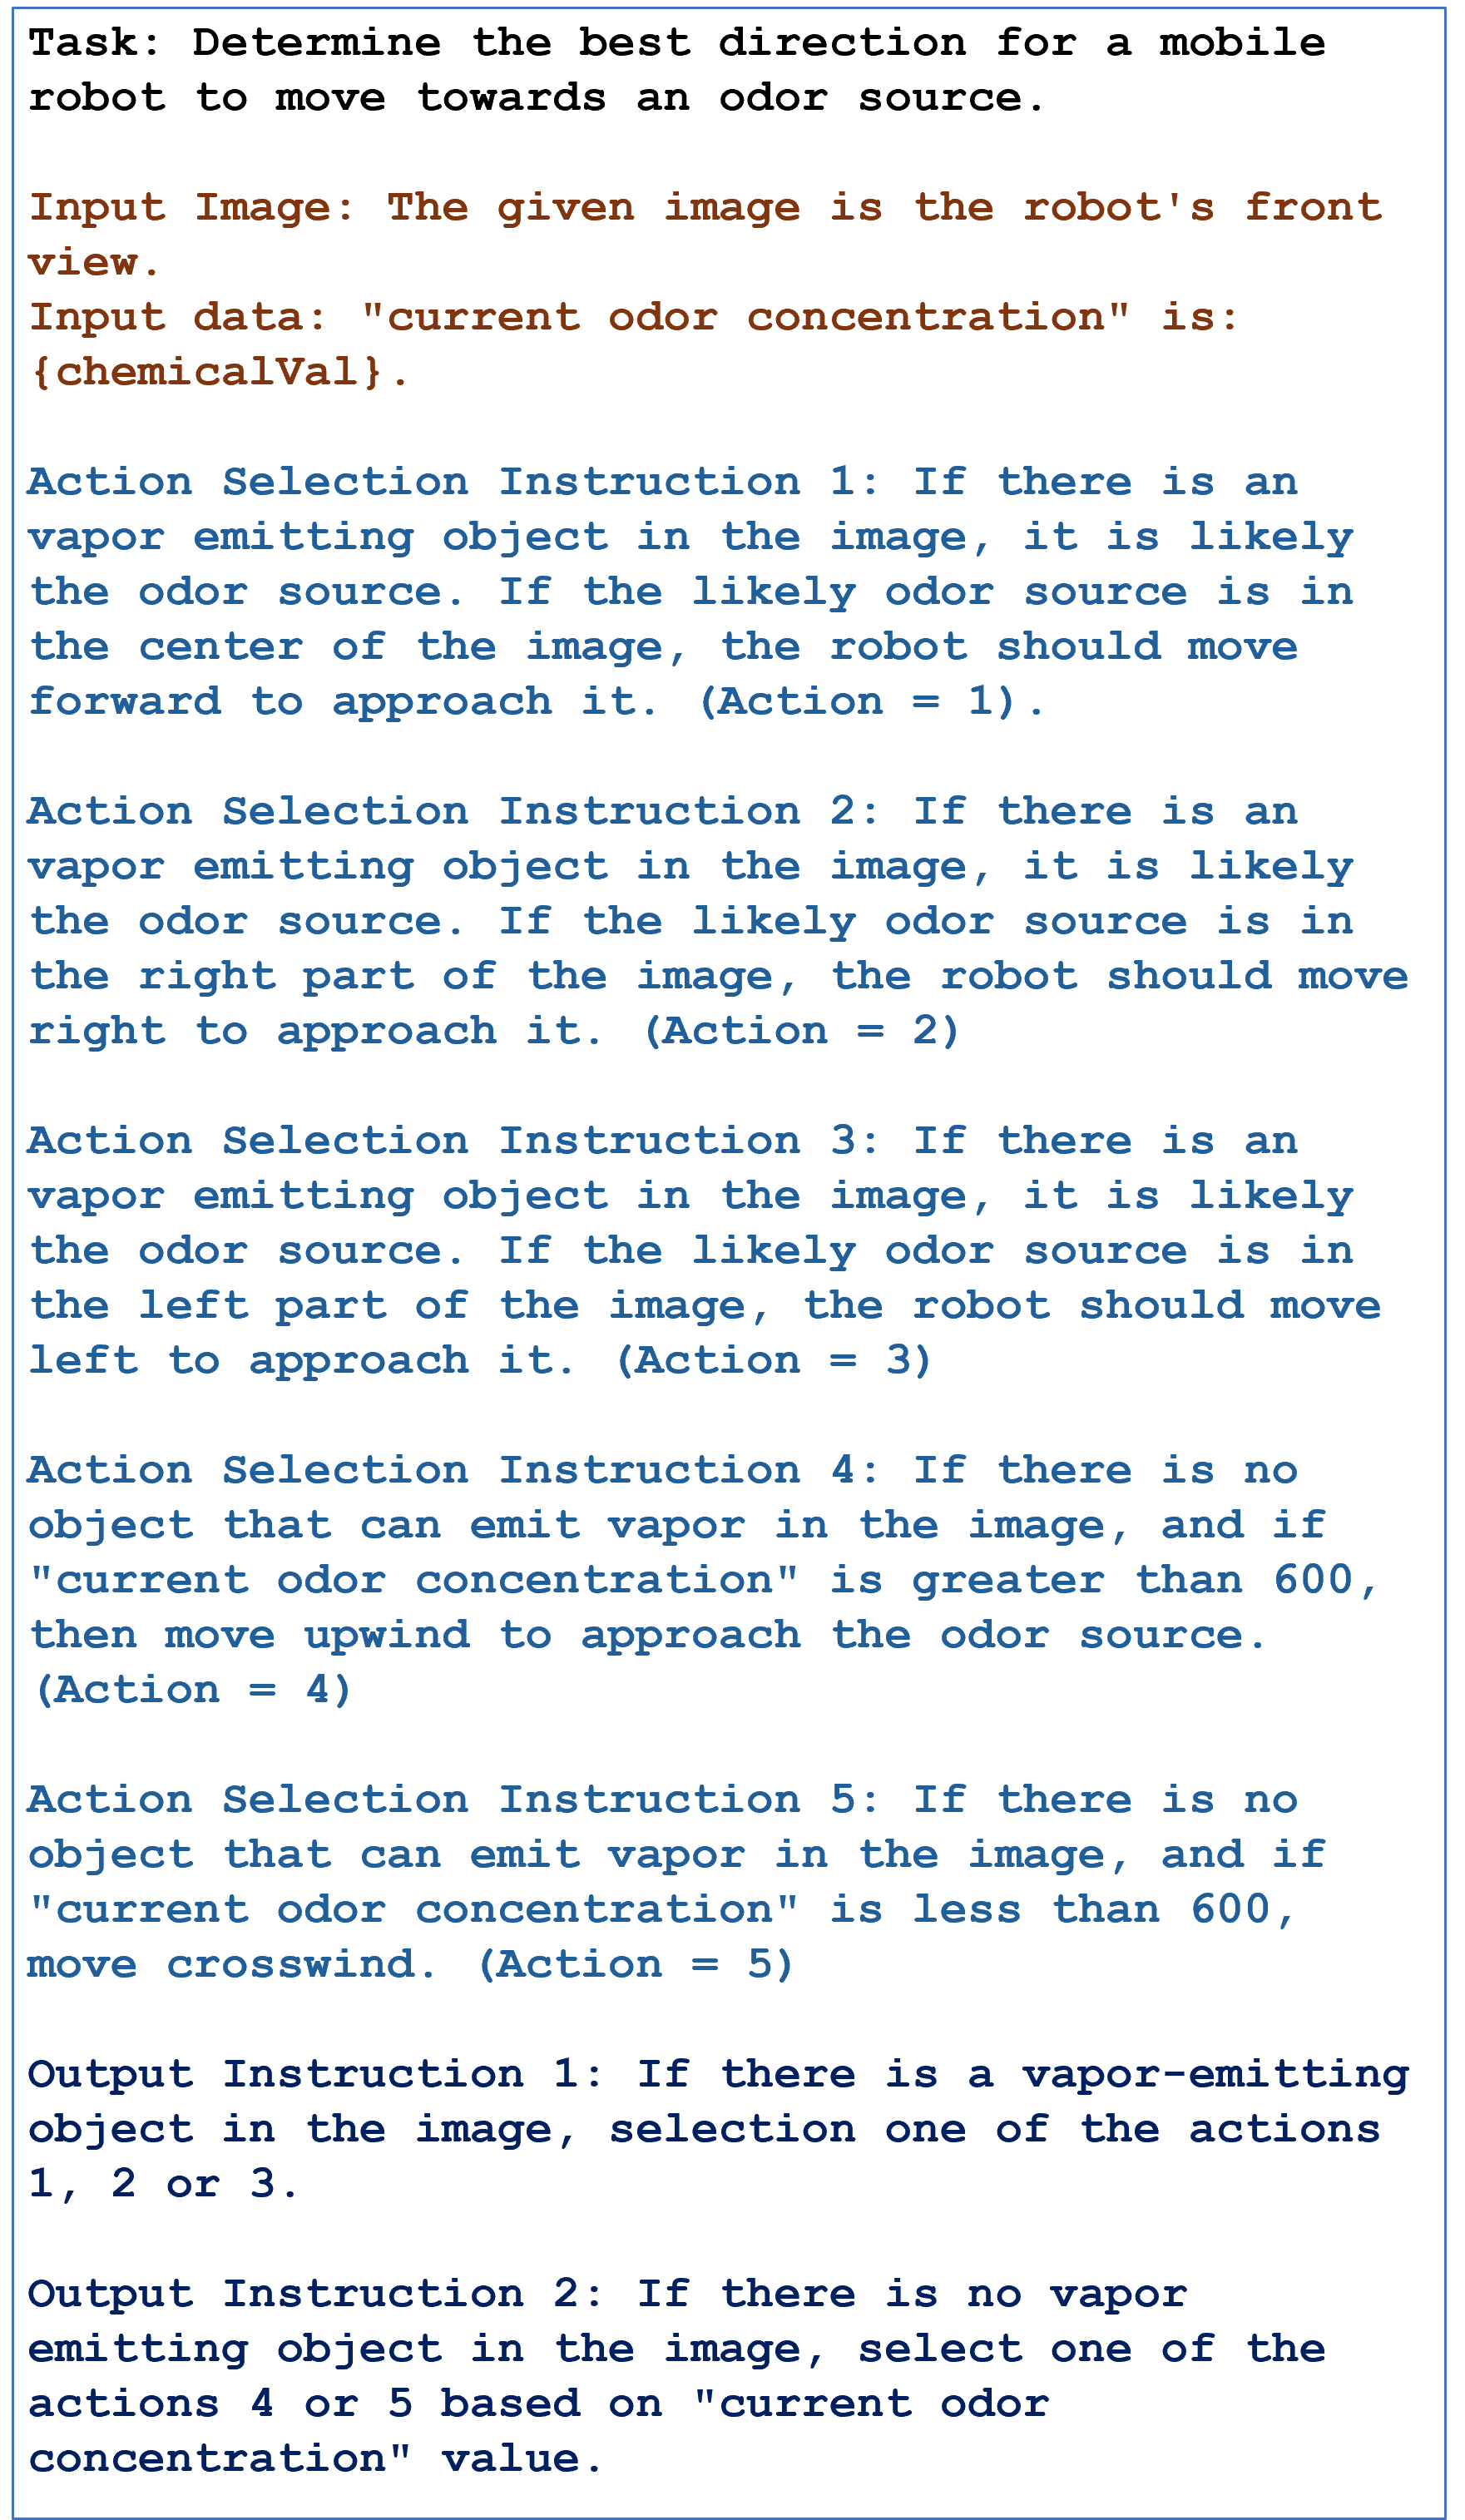
\includegraphics[width=0.7\columnwidth]{Main/Figure/prompt.png}\label{fig:Fprompt}}
\end{center}
\vspace{-.1in}

\caption
{The prompt used to query robot action from GPT-4o multi-modal LLM model.}
%\end{singlespace}
\label{fig:LLMPrompt}
\end{figure}

Figure~\ref{fig:LLMPrompt} shows the prompt used to query robot action from the GPT-4o model. The prompt was developed following the prompt design of the DiLu model \cite{wen2023dilu}. The Task, Action Selection Instructions, and Output Instructions stay the same for every query, only the visual frame and the olfaction reading change with the robot state.

The Task part of the prompt is to communicate the objective of the query with the LLM model. The image is passed to the model without any vision processing. The value of the plume concentration is passed as an integer value.

There are 5 robot actions that the GPT model can select - vision-based `Forward', `Right', `Left' movement, and olfaction-based `Upwind' and `Crosswind' movement. The GPT-4o model is not provided with the name of the odor source object. Rather, it must use reasoning to decide the odor source object from the rest of the objects. Additionally, it needs to utilize its vision and olfaction sensor understanding to determine the best robot action.

\begin{figure}[h!] %% figure
\ \\
\vspace*{-.18in}
\begin{center}
    \subfigure{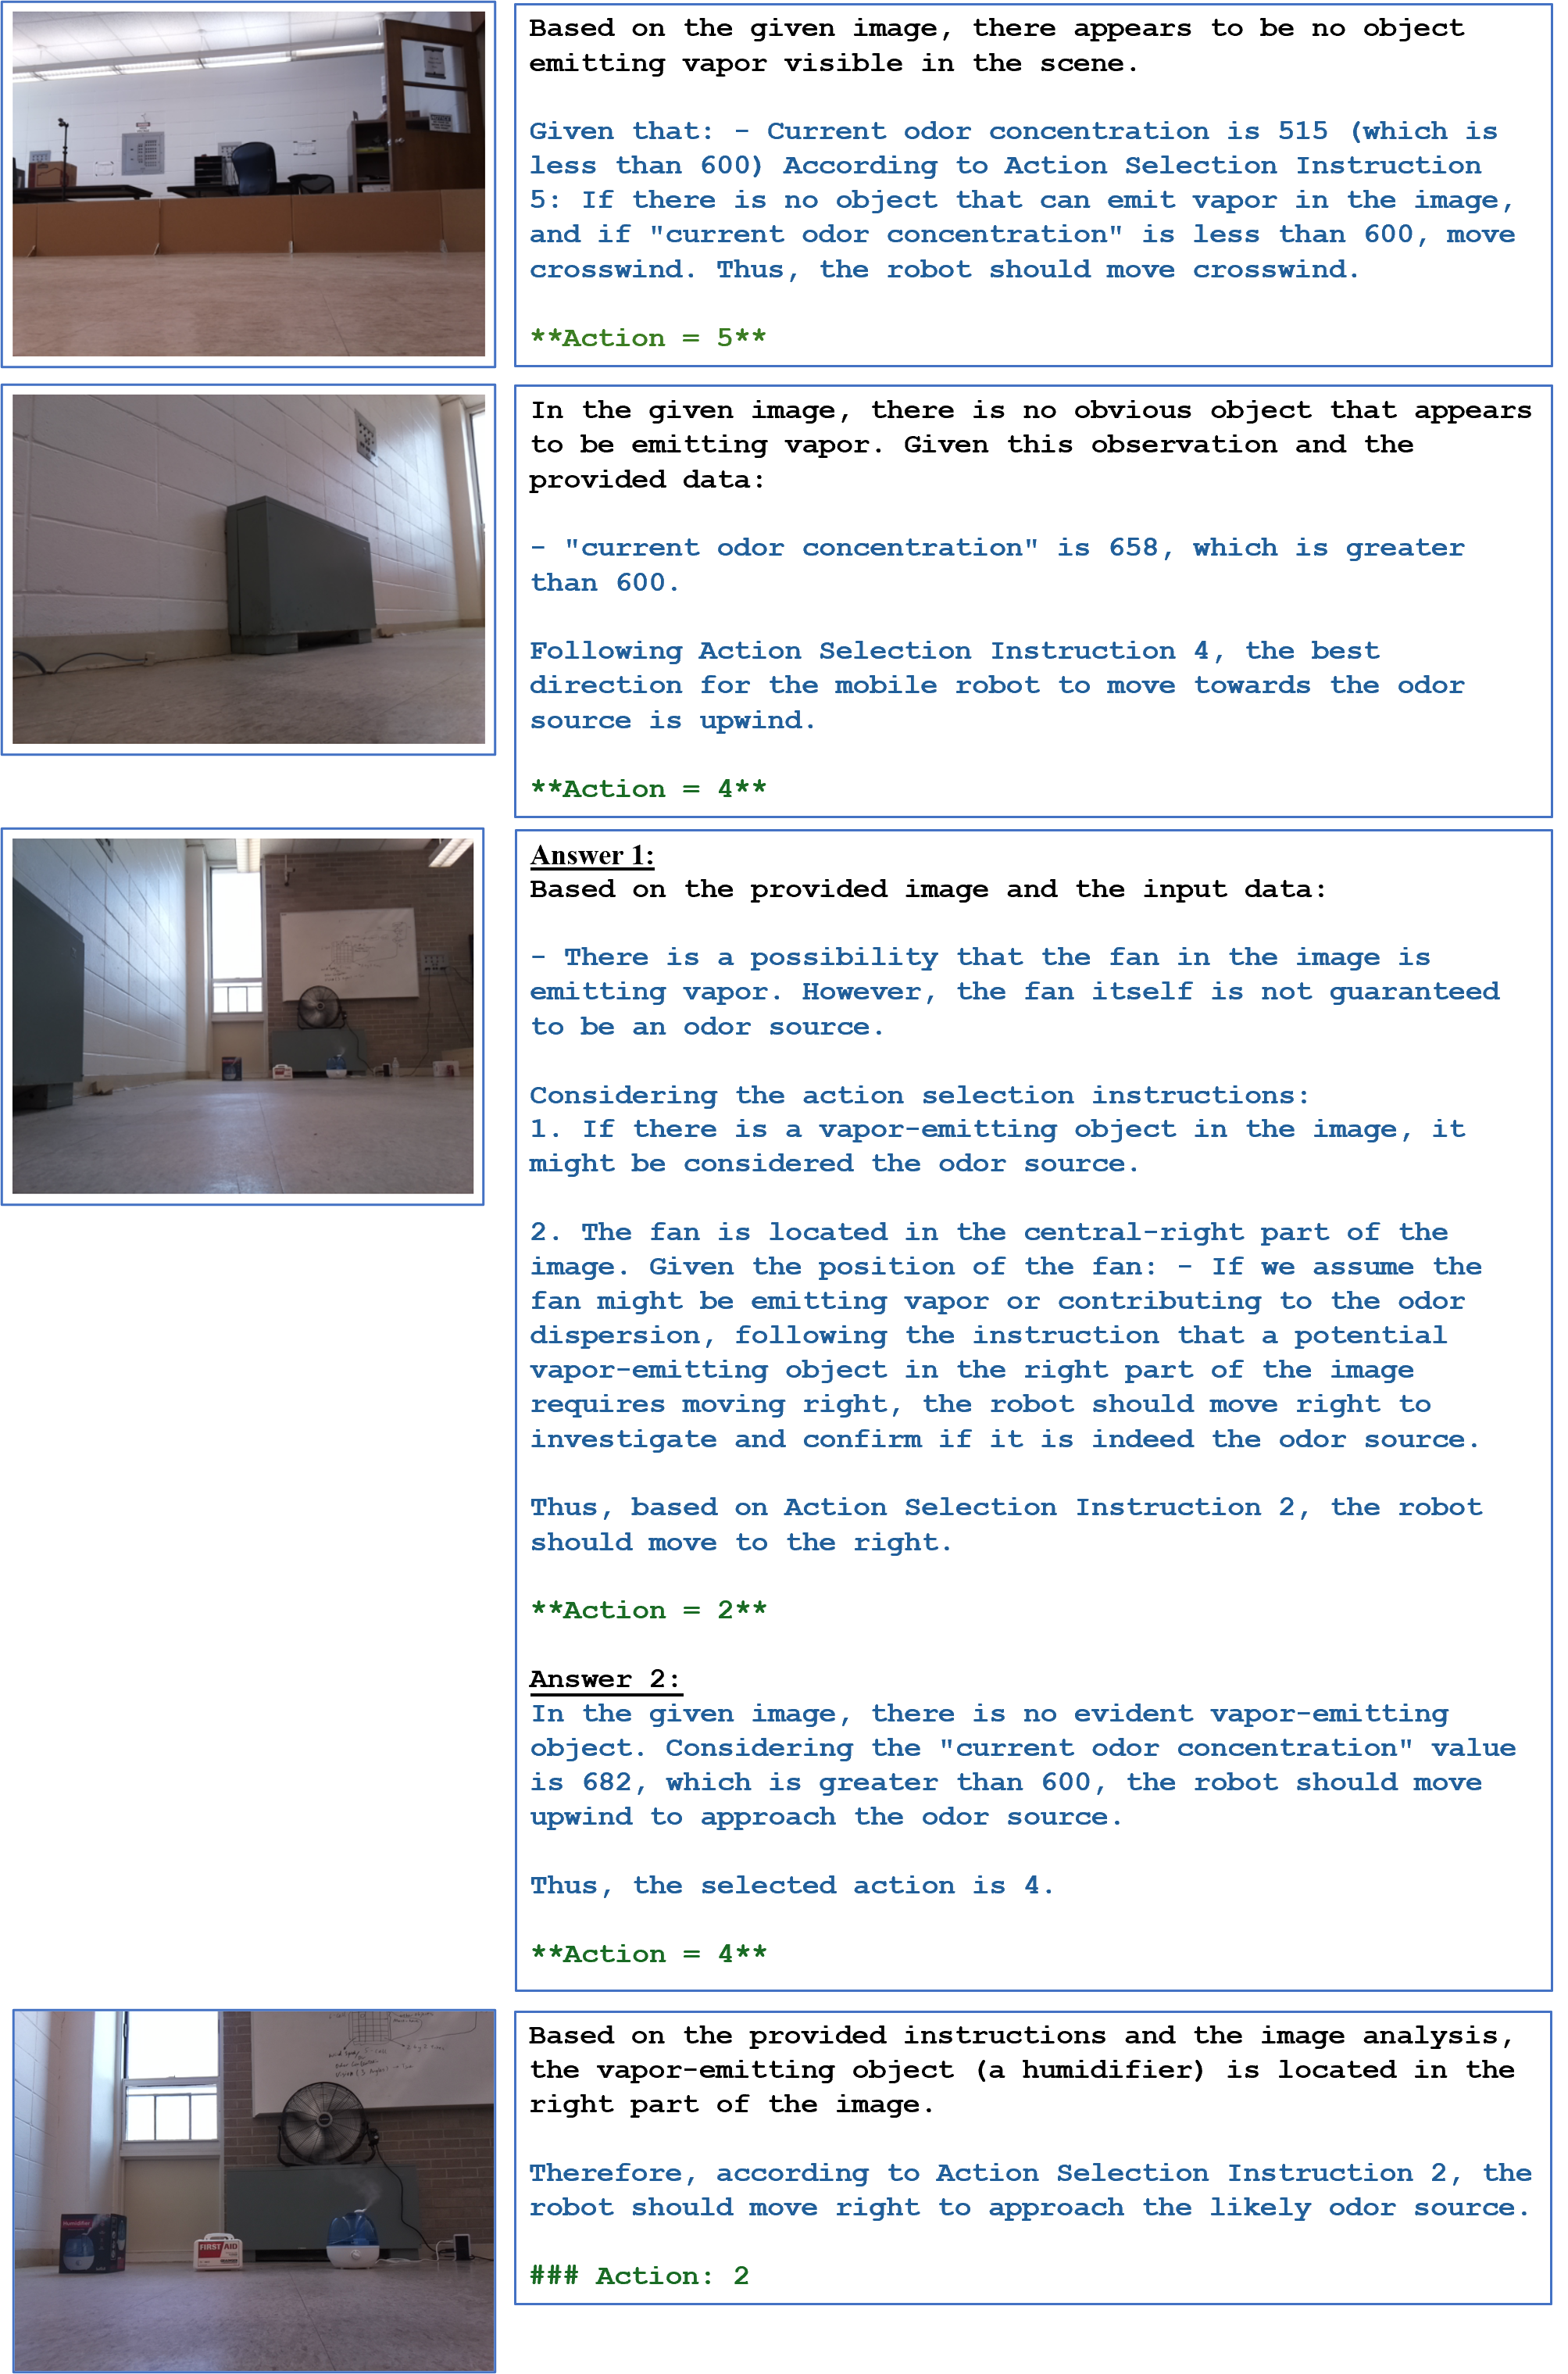
\includegraphics[width=0.8\columnwidth]{Main/Figure/answer.png}\label{fig:Fanswer}}
\end{center}
\vspace{-.1in}

\caption
{GPT-4o chain of thought against the navigation query.}
%\end{singlespace}
\label{fig:LLMAnswers}
\end{figure}

Figure~\ref{fig:LLMAnswers} shows the outputs generated by the GPT-4o model against the navigation queries. In the first query, the GPT model can not see any potential odor source, finds the plume concentration to be lower than the threshold, and correctly selects the `Crosswind' navigation action. In the second query, the model still can not see any potential odor source, finds the plume concentration to be above the threshold, and correctly selects the `Upwind' navigation. In the third query, the odor source is visible. However, the GPT model fails to distinguish the odor source. However, it targets the fan as a potential odor source and selects the correct vision-based action `2'. Upon repeated tests, the same query also generated a wrong action decision of `4' after failing to distinguish the odor source in the visual frame. As the robot approaches closure to the odor source, the GPT model correctly distinguishes the odor source from the other objects (including the humidifier box) and selects the correct action to guide the robot to the odor source.

\subsection{Multi-modal LLM-based ROSL Navigation Algorithm}\label{Subsec:LLMROSLNav}

\begin{figure}[h!] %% figure
\ \\
\vspace*{-.18in}
\begin{center}
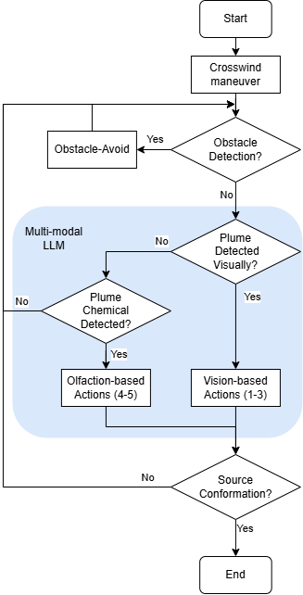
\includegraphics[width=0.5\columnwidth]{Main/Figure/LLMFlow.png}\hspace*{0.04in}
\end{center}
\vspace{-.1in}

\caption
{
The flow diagram of the proposed multi-modal reasoning-based navigation algorithm. There are four navigation behaviors, including `Crosswind maneuver', `Obstacle-Avoid Navigation', `Vision-Based Navigation', and `Olfaction-Based Navigation'.}
%\end{singlespace}
\label{fig:LLM_flow}
\end{figure}

Figure~\ref{fig:LLM_flow} shows the flow diagram of the multi-modal reasoning-based ROSL navigation algorithm. It shares obstacle avoidance and olfaction-based navigation functionalities with the vision and olfaction fusion navigation algorithm discussed in subsection~\ref{Subsec:fusionROSL}. However, the switching between vision and olfaction-based navigation is decided by the multi-modal LLM model.

\section{Experiment}
% ROSL navigation task (same source, platform, search area - vision/navigation-prevnting obstacles, various objects (including fake box) for reasoning, same 2 airflows)
\subsection{Navigation Task}\label{Subsec:LLMNavigationTask}

\begin{figure}[h!]

\ \\
\vspace*{-.18in}

\begin{center}
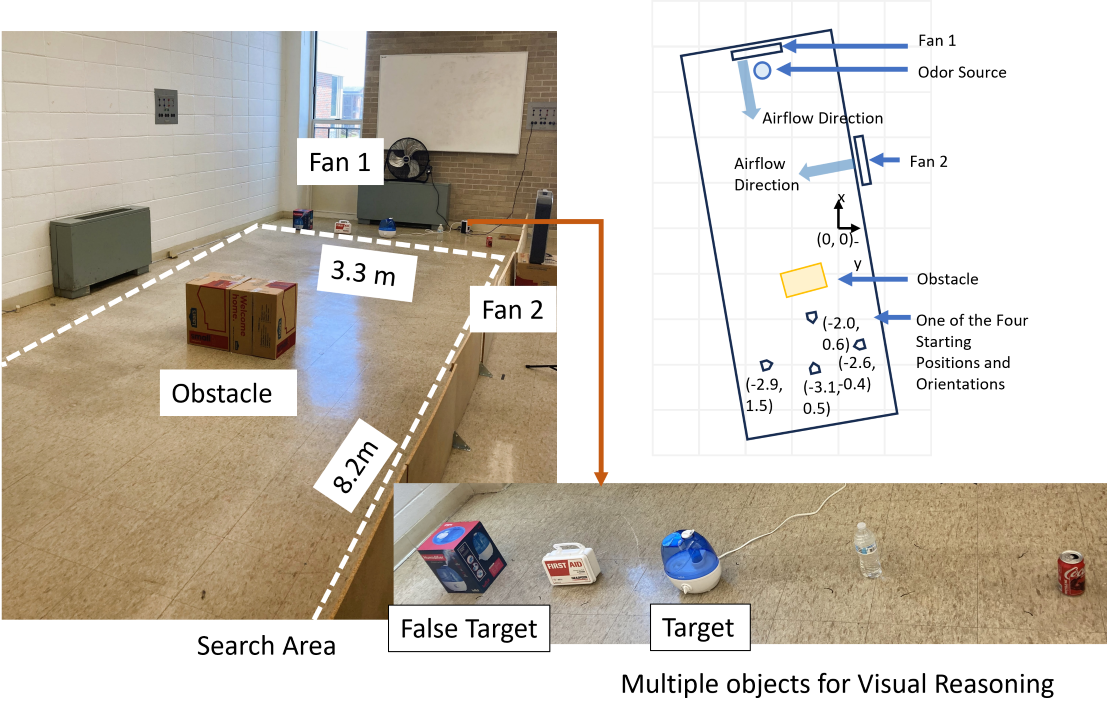
\includegraphics[width=0.9\columnwidth]{Main/Figure/LLMSearchArea.png}\hspace*{0.04in}
\end{center}
\vspace{-.1in}

\caption
{The experimental setup. The robot is initially placed in a downwind area with the objective of finding the odor source. A humidifier loaded with ethanol is employed to generate odor plumes. Two electric fans are placed perpendicularly to create artificial wind fields. An obstacle is placed in the search area. There are 5 objects to test the reasoning capability of the LLM-model.}
%\end{singlespace}
\label{fig:LLMSearchArea}
\end{figure}

The main focus of the experiment is to test the multi-modal reasoning capability of the GPT-4o multi-modal LLM. The experiments use the same search area discussed in subsection~\ref{Sec:fusionExperiment}. Figure~\ref{fig:LLMSearchArea} shows the search area used for ROSL navigation. The search area has an obstacle to block initial odor source vision - the algorithm must select appropriate olfaction-based navigation to approach the odor source at first. Once the algorithm can see the objects, the multi-modal LLM must use reason to understand which object is the valid odor source. An false target, i.e., humidifier box has been added to test the reasoning capability of the multi-modal LLM. 

% Fig~\ref{} shows the search area used for multi-modal-LLM based ROSL navigation experiments. An obstacle placed in the middle of the search area performs two function - 1) it blocks direct visual of the odor source, forcing the robot to follow initial olfaction-based navigation, 2) it tests obstacle avoidance behavior discussed in section~\ref{Subsec:obstacle-avoid}.
% The significant change in this experiment is the addition of various objects depicted in fig~\ref{}.


\subsection{Evaluation Metric}\label{subsec:LLMEvaluationMetric}
The performance of the multimodal-LLM-based ROSL navigation algorithm was compared with the vision and olfaction fusion navigation algorithm discussed in section ~\ref{Subsec:fusionROSL}. %The fusion navigation algorithm can be thought of as an analytical approach to vision and olfaction sensing based ROSL in this case. 
Section~\ref{Sec:fusionResult} showed that the fusion navigation algorithm can successfully localize the odor source using both olfaction and plume vision information. The high testing accuracy of the trained model resulted in accurate plume vision detection from various distances, angles, lighting conditions, etc. On the contrary, the multi-modal LLM model is not trained to know what the odor source object is. Given the goal of the task, the model must - 1) detect objects present in the visual frame, 2) reason from the provided goal which object is the odor source, and 3) select actions that'll guide the robot towards the odor source.

If the average ROSL performance of the multi-modal LLM-based navigation algorithm is not statistically worse than the average ROSL performance of the fusion navigation model, then the multi-modal LLM-based navigation algorithm could be considered a valid ROSL navigation algorithm.

The fusion and multi-modal LLM-based algorithm were tested starting from four positions, and four test runs were recorded from each starting position. In addition to tests conducted in laminar and turbulent airflow environments, as discussed in subsection~\ref{Subsec:fusionNavigationTask}, tests were recorded with one fan directly placed behind the humidifier, inhibiting direct visible plumes to challenge the vision sensing of the fusion and the multi-modal LLM-based algorithms. In total 48 tests were recorded to contrast the two ROSL algorithms.

\section{Results and Discussion}\label{Sec:LLMresults}
% trajectory graphs and tables
% conclusion (generalization, light platforms powered by cloud comutation, training cycle)
\begin{figure}[h!] %% figure
\ \\
\vspace*{-.18in}
\begin{center}
    \subfigure[Fusion env1 pos1]{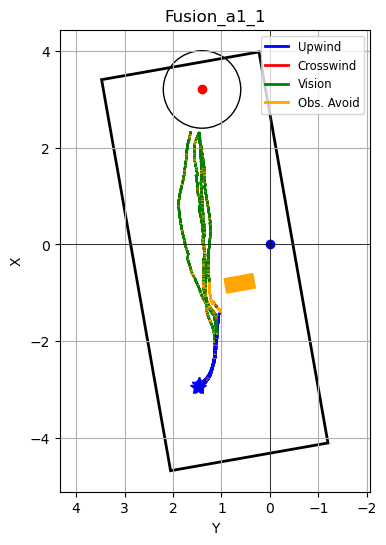
\includegraphics[width=0.24\columnwidth]{Main/Figure/f11.png}\label{fig:Fe1p1}}
    \subfigure[Fusion env1 pos2]{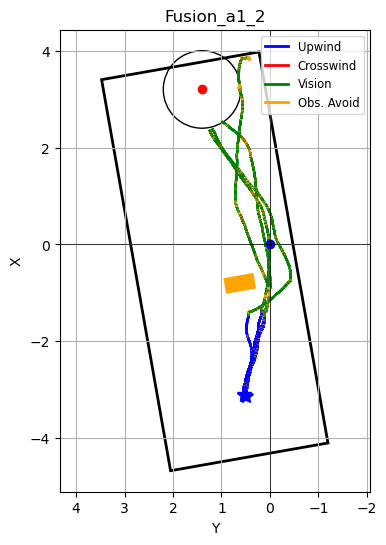
\includegraphics[width=0.24\columnwidth]{Main/Figure/f12.png}\label{fig:Fe1p2}}
    \subfigure[Fusion env1 pos3]{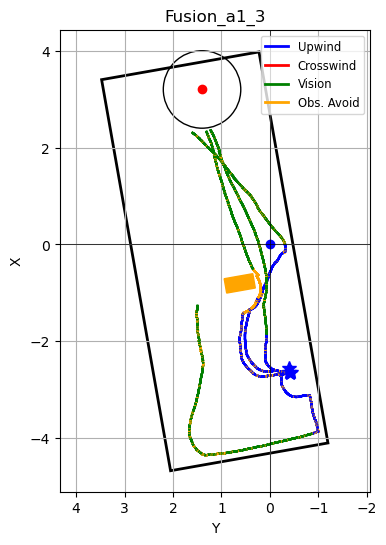
\includegraphics[width=0.24\columnwidth]{Main/Figure/f13.png}\label{fig:Fe1p3}}
    \subfigure[Fusion env1 pos4]{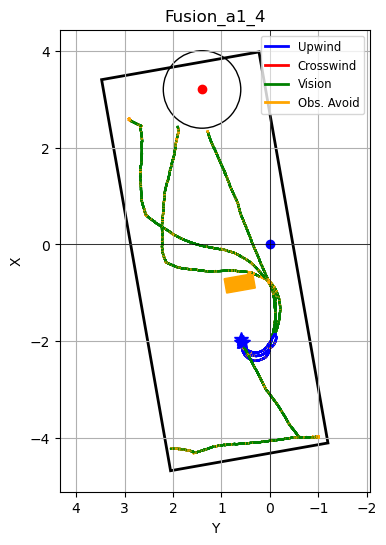
\includegraphics[width=0.24\columnwidth]{Main/Figure/f14.png}\label{fig:Fe1p4}}
    
    \subfigure[LLM env1 pos1]{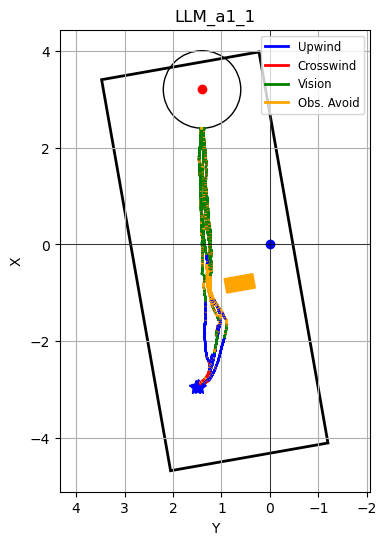
\includegraphics[width=0.24\columnwidth]{Main/Figure/l11.png}\label{fig:Le1p1}}
    \subfigure[LLM env1 pos2]{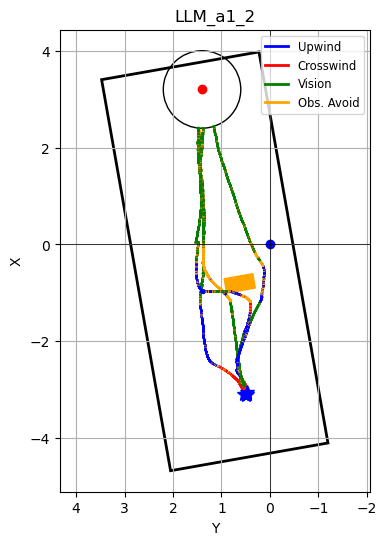
\includegraphics[width=0.24\columnwidth]{Main/Figure/l12.png}\label{fig:Le1p2}}
    \subfigure[LLM env1 pos3]{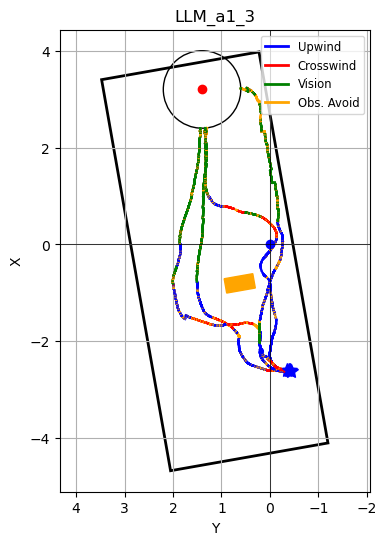
\includegraphics[width=0.24\columnwidth]{Main/Figure/l13.png}\label{fig:Le1p3}}
    \subfigure[LLM env1 pos4]{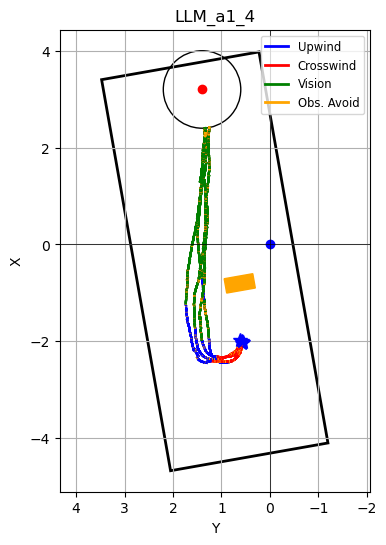
\includegraphics[width=0.24\columnwidth]{Main/Figure/l14.png}\label{fig:Le1p4}}
\end{center}
\vspace{-.1in}

\caption
{Robot trajectories of repeated tests in using fusion navigation algorithm (a$-$d) and multi-modal reasoning-based navigation algorithm (e$-$h) in laminar airflow environment. Four trial runs has been recorded for the four starting positions. The navigation behaviors are: Crosswind, Obstacle-Avoid, Upwind, and Vision-Based Navigation. The obstacle is indicated by orange box, and the odor source is represented by a red point with the surrounding circular source declaration region.}
%\end{singlespace}
\label{fig:LLMe1TrajectoriesLaminar}
\end{figure}

\begin{figure}[h!] %% figure
\ \\
\vspace*{-.18in}
\begin{center}
    \subfigure[Fusion env2 pos1]{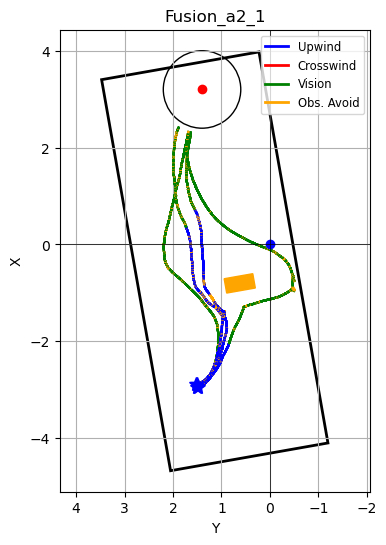
\includegraphics[width=0.24\columnwidth]{Main/Figure/f21.png}\label{fig:Fe2p1}}
    \subfigure[Fusion env2 pos2]{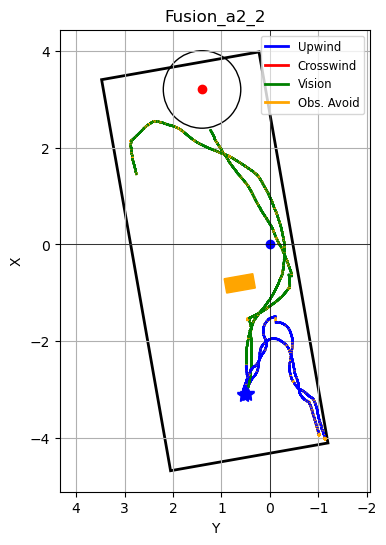
\includegraphics[width=0.24\columnwidth]{Main/Figure/f22.png}\label{fig:Fe2p2}}
    \subfigure[Fusion env2 pos3]{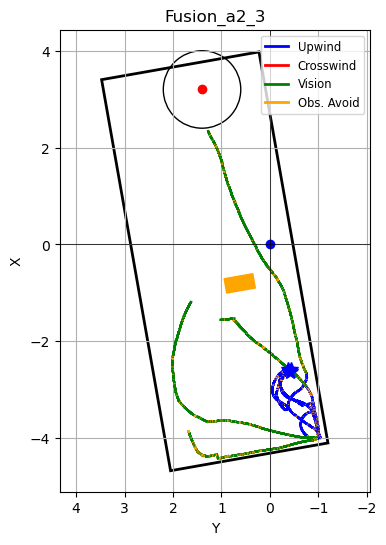
\includegraphics[width=0.24\columnwidth]{Main/Figure/f23.png}\label{fig:Fe2p3}}
    \subfigure[Fusion env2 pos4]{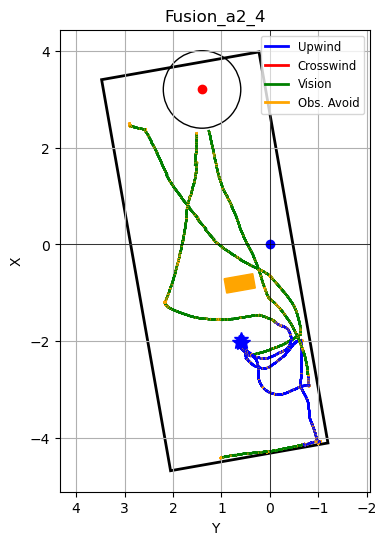
\includegraphics[width=0.24\columnwidth]{Main/Figure/f24.png}\label{fig:Fe2p4}}
    
    \subfigure[LLM env2 pos1]{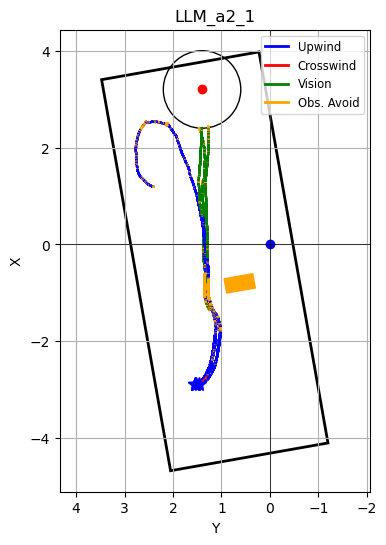
\includegraphics[width=0.24\columnwidth]{Main/Figure/l21.png}\label{fig:Le2p1}}
    \subfigure[LLM env2 pos2]{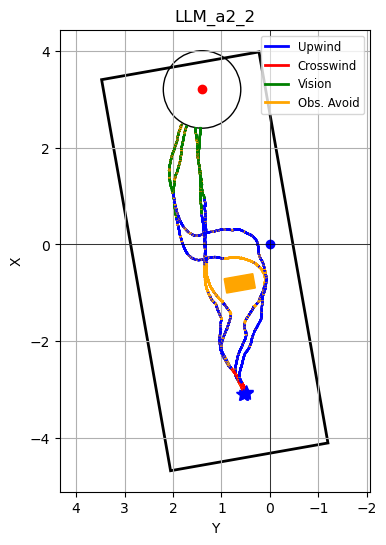
\includegraphics[width=0.24\columnwidth]{Main/Figure/l22.png}\label{fig:Le2p2}}
    \subfigure[LLM env2 pos3]{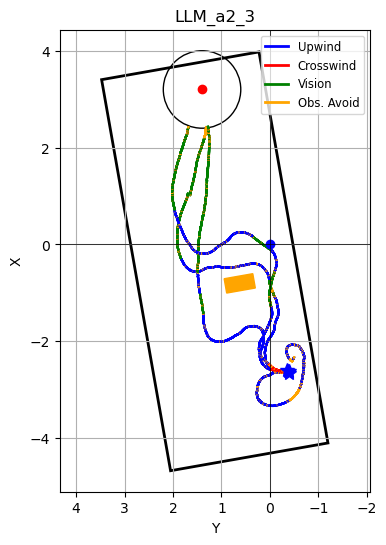
\includegraphics[width=0.24\columnwidth]{Main/Figure/l23.png}\label{fig:Le2p3}}
    \subfigure[LLM env2 pos4]{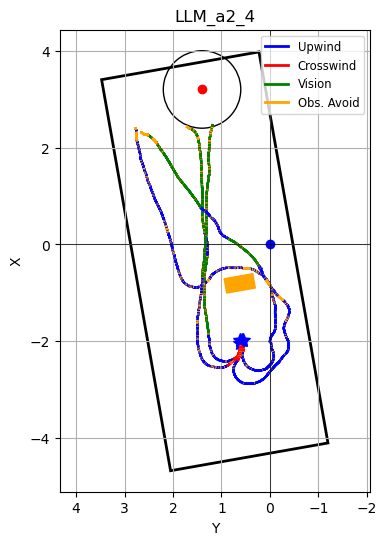
\includegraphics[width=0.24\columnwidth]{Main/Figure/l24.png}\label{fig:Le2p4}}
\end{center}
\vspace{-.1in}

\caption
{Robot trajectories of repeated tests in using fusion navigation algorithm (a$-$d) and multi-modal reasoning-based navigation algorithm (e$-$h) in turbulent airflow environment. Four trial runs has been recorded for the four starting positions. The navigation behaviors are: Crosswind, Obstacle-Avoid, Upwind, and Vision-Based Navigation. The obstacle is indicated by orange box, and the odor source is represented by a red point with the surrounding circular source declaration region.}
%\end{singlespace}
\label{fig:LLMe1TrajectoriesTurbulent}
\end{figure}


\begin{table}[h]
\caption{Comparison of Average Search Time, Travelled Distance, and Success Rate of the validated Vision and Olfaction Fusion Navigation algorithm and the proposed Multi-modal Reasoning-based Navigation algorithm.}
\label{tab:LLM_expeiment_result}
\ \\
\centerline{
\begin{tabular}{|c|c|ccc|ccc|}
\hline
\multirow{2}{*}{\textbf{\begin{tabular}[c]{@{}c@{}}Airflow\\ Env.\end{tabular}}} & \multirow{2}{*}{\textbf{\begin{tabular}[c]{@{}c@{}}Start\\ Pos.\end{tabular}}} & \multicolumn{3}{c|}{\textbf{\begin{tabular}[c]{@{}c@{}}Vision and Olfaction\\ Fusion Navigation\\ Algorithm\end{tabular}}}                                                                                                                                                    & \multicolumn{3}{c|}{\textbf{\begin{tabular}[c]{@{}c@{}}Multi-modal\\ Reasoning-based\\ Navigation\\ Algorithm\end{tabular}}}                                                                                                                                                  \\ \cline{3-8} 
                                                                                 &                                                                                & \multicolumn{1}{c|}{\textbf{\begin{tabular}[c]{@{}c@{}}Avg.\\ Search\\ Time\\ (s)\end{tabular}}} & \multicolumn{1}{c|}{\textbf{\begin{tabular}[c]{@{}c@{}}Avg.\\ Travel-\\ led\\ Dist.\\ (m)\end{tabular}}} & \textbf{\begin{tabular}[c]{@{}c@{}}Success\\ Rate\end{tabular}} & \multicolumn{1}{c|}{\textbf{\begin{tabular}[c]{@{}c@{}}Avg.\\ Search\\ Time\\ (s)\end{tabular}}} & \multicolumn{1}{c|}{\textbf{\begin{tabular}[c]{@{}c@{}}Avg.\\ Travel-\\ led\\ Dist.\\ (m)\end{tabular}}} & \textbf{\begin{tabular}[c]{@{}c@{}}Success\\ Rate\end{tabular}} \\ \hline
\multirow{4}{*}{\textbf{Laminar}}                                                & \begin{tabular}[c]{@{}c@{}}(-2.9,\\ 1.5)\end{tabular}                          & \multicolumn{1}{c|}{\textbf{72.5}}                                                               & \multicolumn{1}{c|}{\textbf{5.56}}                                                                       & \textbf{1.0}                                                    & \multicolumn{1}{c|}{75.2}                                                                        & \multicolumn{1}{c|}{5.7}                                                                                 & 1.0                                                             \\ \cline{2-8} 
                                                                                 & \begin{tabular}[c]{@{}c@{}}(-3.1,\\ 0.5)\end{tabular}                          & \multicolumn{1}{c|}{81.4}                                                                        & \multicolumn{1}{c|}{6.2}                                                                                 & 0.75                                                            & \multicolumn{1}{c|}{\textbf{80.9}}                                                               & \multicolumn{1}{c|}{\textbf{6.1}}                                                                        & \textbf{1.0}                                                    \\ \cline{2-8} 
                                                                                 & \begin{tabular}[c]{@{}c@{}}(-2.6,\\ -0.4)\end{tabular}                         & \multicolumn{1}{c|}{\textbf{89.7}}                                                               & \multicolumn{1}{c|}{\textbf{6.2}}                                                                        & 0.75                                                            & \multicolumn{1}{c|}{90.5}                                                                        & \multicolumn{1}{c|}{6.7}                                                                                 & \textbf{1.0}                                                    \\ \cline{2-8} 
                                                                                 & \begin{tabular}[c]{@{}c@{}}(-2.0,\\ 0.6)\end{tabular}                          & \multicolumn{1}{c|}{93.2}                                                                        & \multicolumn{1}{c|}{6.5}                                                                                 & 0.5                                                             & \multicolumn{1}{c|}{\textbf{74.7}}                                                               & \multicolumn{1}{c|}{\textbf{5.9}}                                                                        & \textbf{1.0}                                                    \\ \hline
\multirow{4}{*}{\textbf{Turbulent}}                                              & \begin{tabular}[c]{@{}c@{}}(-2.9,\\ 1.5)\end{tabular}                          & \multicolumn{1}{c|}{87.8}                                                                        & \multicolumn{1}{c|}{6.3}                                                                                 & \textbf{1.0}                                                    & \multicolumn{1}{c|}{\textbf{76.2}}                                                               & \multicolumn{1}{c|}{\textbf{5.6}}                                                                        & 0.75                                                            \\ \cline{2-8} 
                                                                                 & \begin{tabular}[c]{@{}c@{}}(-3.1,\\ 0.5)\end{tabular}                          & \multicolumn{1}{c|}{91.9}                                                                        & \multicolumn{1}{c|}{6.6}                                                                                 & 0.25                                                            & \multicolumn{1}{c|}{\textbf{87.6}}                                                               & \multicolumn{1}{c|}{\textbf{6.5}}                                                                        & \textbf{1.0}                                                    \\ \cline{2-8} 
                                                                                 & \begin{tabular}[c]{@{}c@{}}(-2.6,\\ -0.4)\end{tabular}                         & \multicolumn{1}{c|}{100.7}                                                                       & \multicolumn{1}{c|}{\textbf{7.4}}                                                                        & 0.25                                                            & \multicolumn{1}{c|}{\textbf{97.5}}                                                               & \multicolumn{1}{c|}{7.4}                                                                                 & \textbf{0.75}                                                   \\ \cline{2-8} 
                                                                                 & \begin{tabular}[c]{@{}c@{}}(-2.0,\\ 0.6)\end{tabular}                          & \multicolumn{1}{c|}{110.7}                                                                       & \multicolumn{1}{c|}{8.0}                                                                                 & \textbf{0.5}                                                    & \multicolumn{1}{c|}{\textbf{79.8}}                                                               & \multicolumn{1}{c|}{\textbf{5.9}}                                                                        & 0.5                                                             \\ \hline
\end{tabular}
}

\ \\
\vspace{-.1in}

\end{table}

\textcolor{black}{Subsection~\ref{Subsec:LLMPrompt} showed that GPT-4o can make a few errors in vison-based action selection. However, the combination of olfaction and vision-based navigation takes the robot closer to the odor source, which improves visual sensing of the odor source and thus reduces the errors in visual reasoning.}

Figure~\ref{fig:LLMe1TrajectoriesLaminar} shows trajectories of the multi-modal reasoning based algorithm in a laminar airflow environment. Figure~\ref{fig:LLMe1TrajectoriesTurbulent} shows trajectories turbulent airflow environment. There were four starting positions in this setup, and four trial runs were recorded for each starting position. Table~\ref{tab:LLM_expeiment_result} shows the performance comparison results. The multi-modal reasoning-based navigation algorithm performed better than the vision and olfaction fusion navigation algorithm in a laminar airflow environment in terms of average success rate, (100\% vs 75\%) and average traveled distance (traveled less distance from 3 starting points vs from 1 starting point). The Multi-modal Reasoning-based navigation algorithm also performed better than the Fusion navigation algorithm in a turbulent airflow environment in terms of average success rate (75\% vs 50\%), average travel time (took less time from all 4 starting points), and average traveled distance (traveled less distance from three starting points, and traveled the equal distance from one starting point). The multi-modal reasoning-based algorithm follows more efficient vision-based navigation behavior even if the odor source is not completely discerned in the visual frame. This gives the navigation algorithm an advantage over the fusion navigation algorithm.

However, their mean difference is not statistically significant at a 5\% confidence level (p-value is 0.16). Given the Fusion model is already validated, the search performance of the multi-modal reasoning model is validated.
